\section{Dataset Collection Protocol}
\label{appendix:dataset_details}

\noindent\textit{This appendix describes the random-exploration dataset used for world model
training (Appendix~\ref{appendix:world_model}). The 333k post-recalibration dataset used
for IQL training is described in Appendix~\ref{appendix:offline_rl}. The
experimental evaluation protocol (stratified benchmarking) is in
Appendix~\ref{appendix:protocol}.}

\begin{figure}[H]
  \centering
  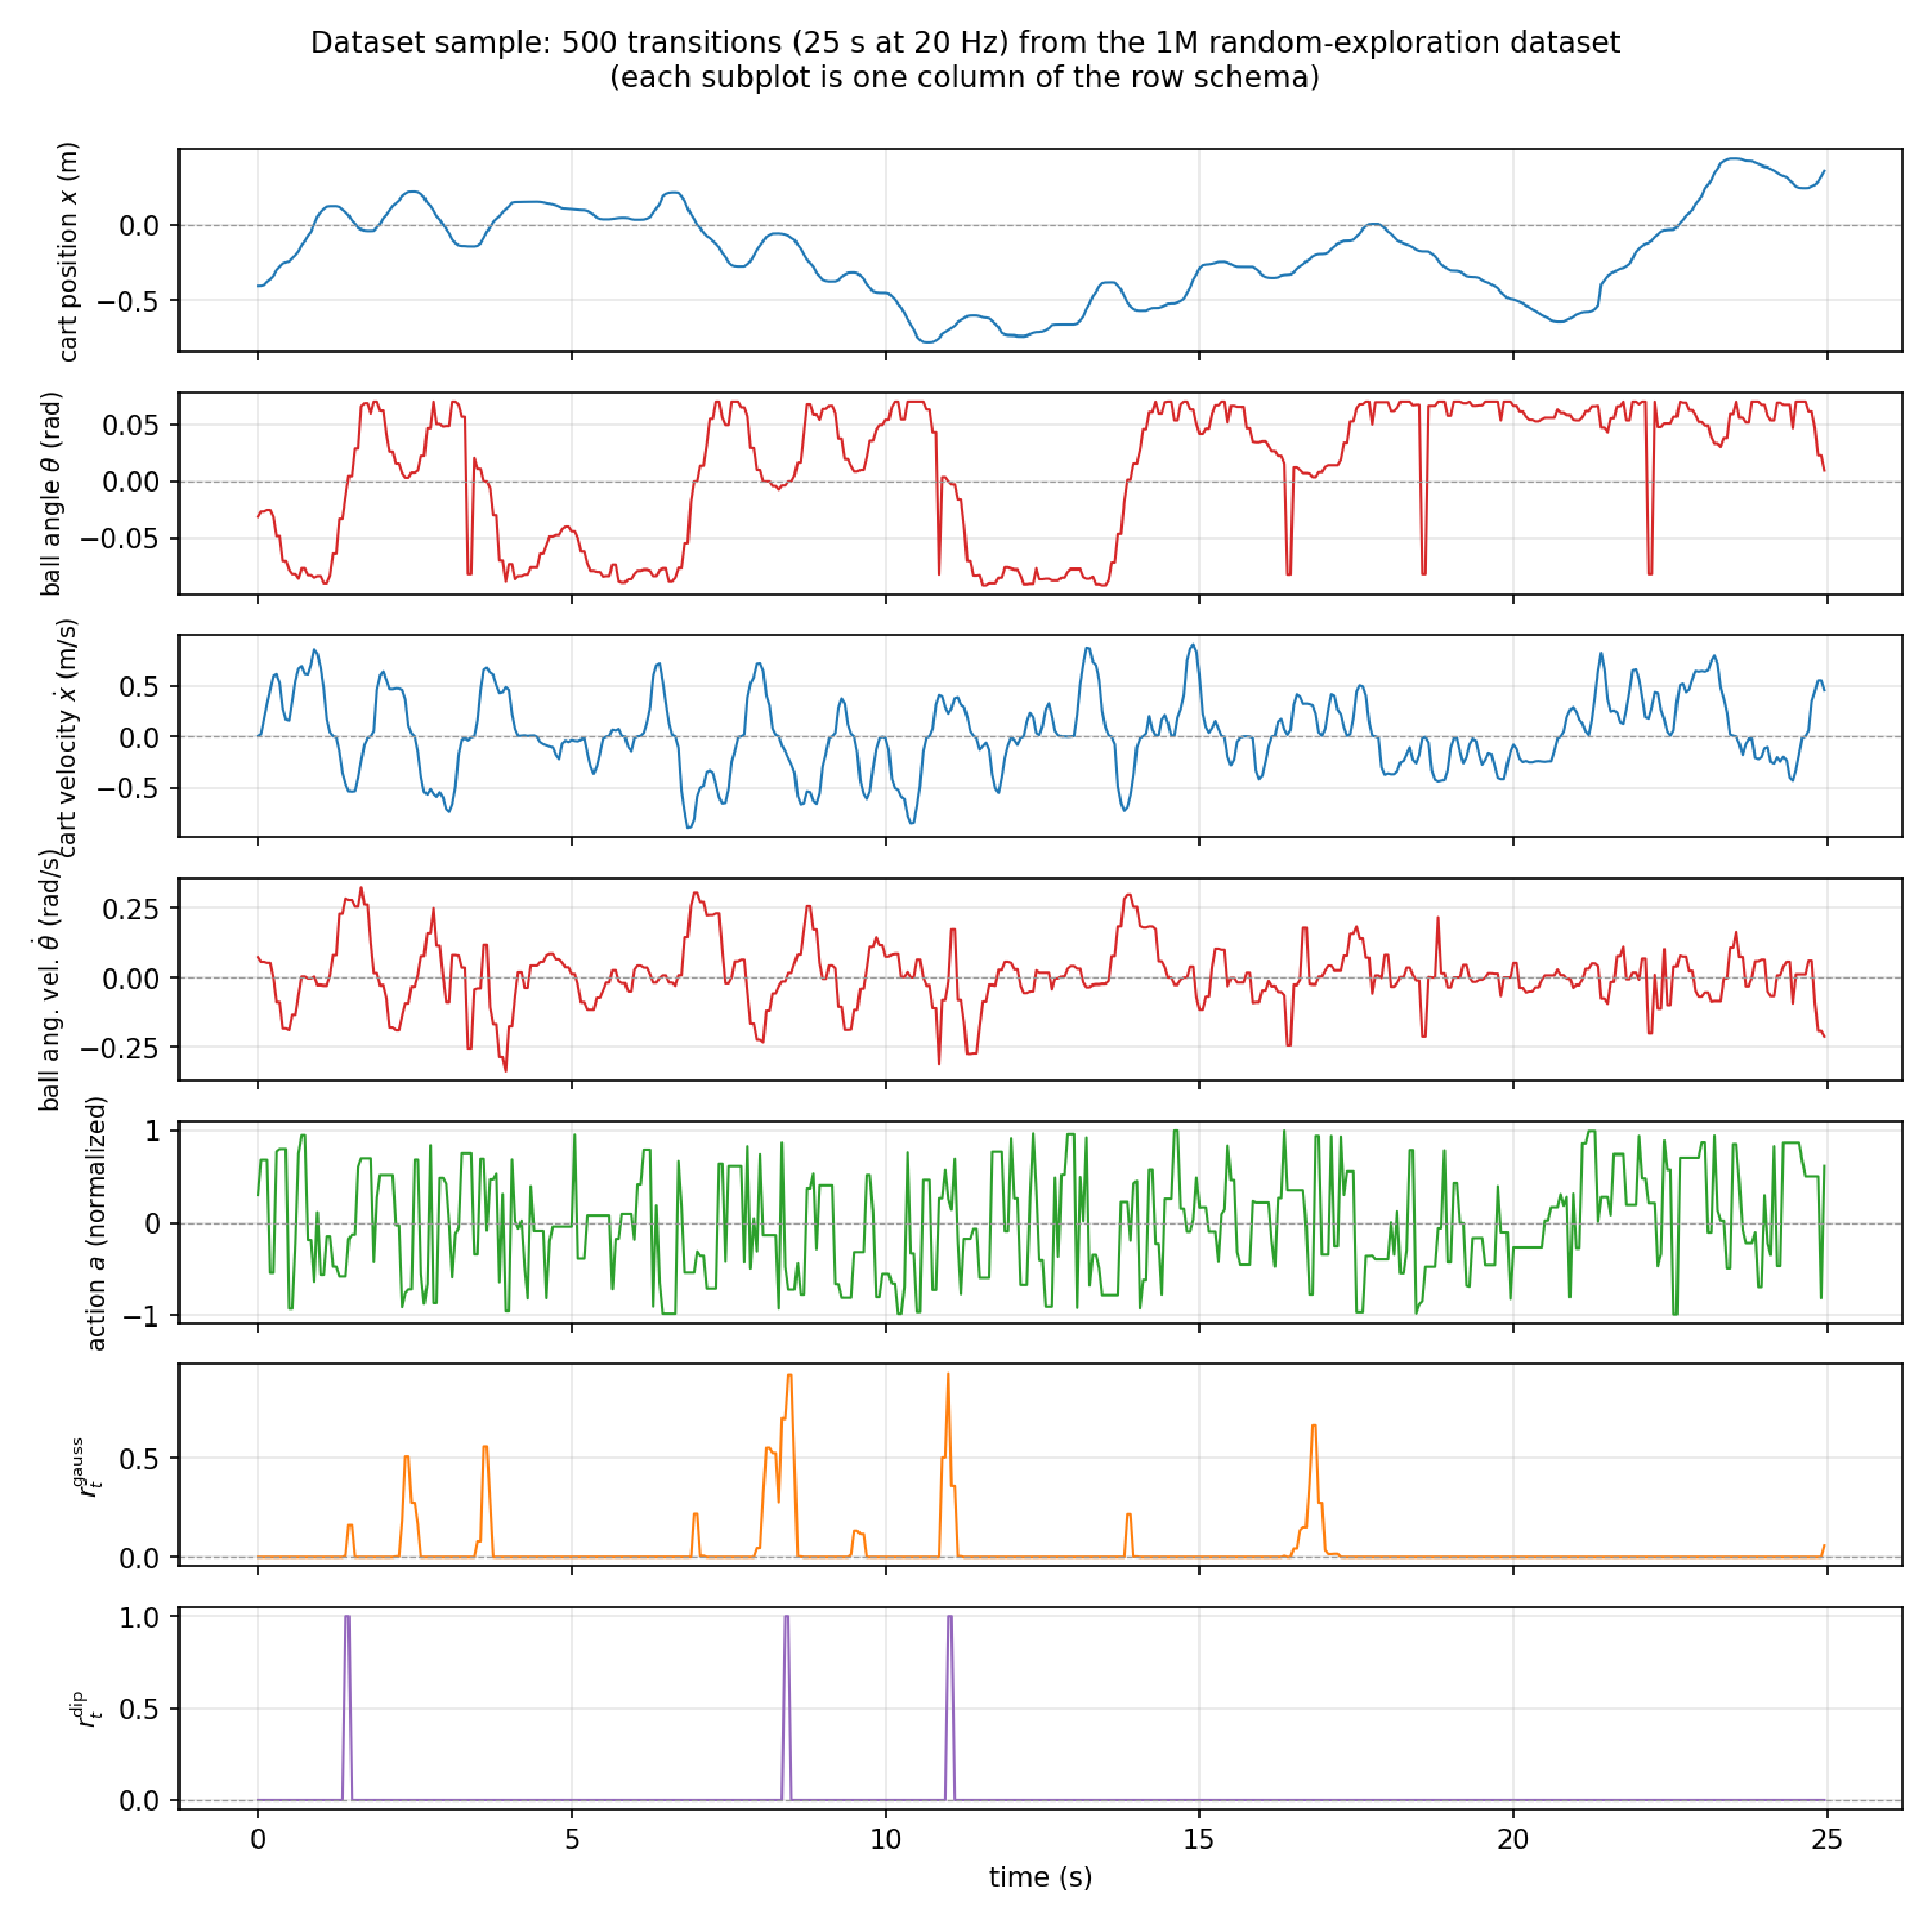
\includegraphics[width=0.98\columnwidth]{figures/dataset_sample.eps}
  \caption{A 500-transition contiguous sample of the 1M
    random-exploration dataset (row schema of
    Eq.~\ref{eq:dataset_row}), plotted as a time series at the 20\,Hz
    control rate. Each subplot is one variable of the row: cart position
    $x$, ball angle $\theta$, cart velocity $\dot{x}$, ball angular
    velocity $\dot{\theta}$, the action $a$ (plotted normalized to
    $[-1,1]$), the Gaussian position reward $r^{\mathrm{gauss}}_t$, and the
    binary IR-dip reward $r^{\mathrm{dip}}_t$ (the hardware IR dip-sensor
    bit, 1 while the sensor reports the ball over the central dip).}
  \label{fig:dataset_sample}
\end{figure}

We recorded random trajectories covering the full state space to
support downstream tasks such as system identification, offline RL,
and learning-based world modeling, collecting separate datasets for
discrete and continuous actions. The agent's normalized action
($\{-1, 0, +1\}$ discrete, $[-1,1]$ continuous) maps to a physical
cart-velocity command ($\{-0.9, 0, +0.9\}$ and $[-0.9, 0.9]$\,m/s). The
stored $a_t$ depends on the collection: the calibrated 1M files store this
m/s command, while the earlier \texttt{pre\_neg} collection stores the
normalized action in $[-1,1]$.
Each row contains:
\begin{equation}
\label{eq:dataset_row}
[x_t,\, \dot{x}_t,\, \theta_t,\, \dot{\theta}_t,\; a_t,\;
 x_{t+1},\, \dot{x}_{t+1},\, \theta_{t+1},\, \dot{\theta}_{t+1},\;
 r^\text{gauss}_t,\; r^\text{dip}_t],
\end{equation}
where
\begin{align}
r^\text{gauss}_t &=
  \exp\!\Bigl(-\frac{\theta_t^2}{2\sigma_r^2}\Bigr)
  \cdot
  \exp\!\Bigl(-\frac{|\dot{\theta}_t|}{v_\text{scale}}\Bigr),
\\
r^\text{dip}_t &=
\begin{cases}
1, & |\theta_{t+1}| \le \theta_\text{center} \\
0, & \text{otherwise.}
\end{cases}
\end{align}
Here $\sigma_r = \theta_\text{max}/16 \approx 0.005$\,rad sets the width
of the Gaussian position reward ($\theta_\text{max}$ is the ball angular
limit, 0.081\,rad in the calibrated collections and 0.075 in
\texttt{pre\_neg}), $v_\text{scale} = 0.2$\,rad/s scales the
angular-velocity term, and $\theta_\text{center} = 0.007$\,rad
(about 15\,mm of arc at $R = 2.101$\,m) is the dip half-band. In the 1M
random-exploration files, the stored $r^\text{dip}_t$ column is the raw
hardware IR dip-sensor bit read from the serial stream; the angular form
above, evaluated on the next-state angle $\theta_{t+1}$, is the offline
recomputation applied when rebuilding the 333k post-recalibration dataset
(\texttt{build\_flat\_dataset.py}).
We recorded over one million steps for the random-exploration
dataset used for world model training, stored in compressed HDF5
format, with the full acquisition scripts available in the public
repository. The two released 1M collections differ in layout: the
calibrated files (\texttt{calib196\_148}, \texttt{calib196\_160}) add four
raw time-of-flight columns (previous and current \texttt{raw\_left\_mm} and
\texttt{raw\_right\_mm}) for a 15-column on-disk array, while the earlier
\texttt{pre\_neg} collection is the 11-column form of
Eq.~\ref{eq:dataset_row}. The world-model loader reads only the
four-element state, the action, and the four-element next state.

Figure~\ref{fig:dataset_sample} shows a 500-transition contiguous
sample from the 1M random-exploration dataset, one subplot per variable
in the row schema of Eq.~\ref{eq:dataset_row}, giving a visual sense of
what one dataset ``looks like'' as a time series (the caption details
each channel).

We used the 1M-transition random-exploration dataset
exclusively to train the LSTM world model
(Appendix~\ref{appendix:world_model}),
which is then used by MPPI and PPO-WM (two checkpoints trained on
two 1\,M collections; see Appendix~\ref{appendix:wm_provenance}). It is \emph{not} used
for offline RL training, because random actions provide insufficient
coverage of successful recovery behavior for an offline policy.
IQL instead uses a separate post-recalibration dataset (333{,}497
transitions from 1{,}415 mixed-controller hardware trials, rewards
recomputed offline), detailed in Appendix~\ref{appendix:offline_rl}. It
is available as \texttt{arcball\_post\_recalib\_flat.h5} (built by
\texttt{data/build\_flat\_dataset.py}).

\subsection{Data-Collection Notes}
\label{appendix:dataset_notes}

Two practical lessons from collecting these datasets on real hardware are
worth recording, since both bear directly on data quality downstream.

\textbf{Solder the sensor wiring:} connect the time-of-flight sensors to the
Arduino with soldered joints rather than push-fit jumper or breadboard
connections. During random exploration the ball strikes the arc walls
repeatedly, and the resulting vibration gradually loosens push-fit
connectors. A momentarily broken power or signal line produces dropped or
frozen readings that are easy to miss during a long unattended collection
run; a soldered harness removes this failure mode.

\textbf{Inspect trajectories before training:} visualize the recorded state
variables before committing a dataset to training. A sensor channel can go
dead partway through a run and hold a constant or otherwise invalid value
that still passes the on-line validity checks, so the fault survives into
the stored data. Plotting each state variable as a time series (as in
Figure~\ref{fig:dataset_sample}) makes such segments immediately visible;
training on them silently degrades the world model and any policy learned
downstream.
